\section[\textit{Erratum}]{\textit{Erratum}}
\begin{figure}
\centering 
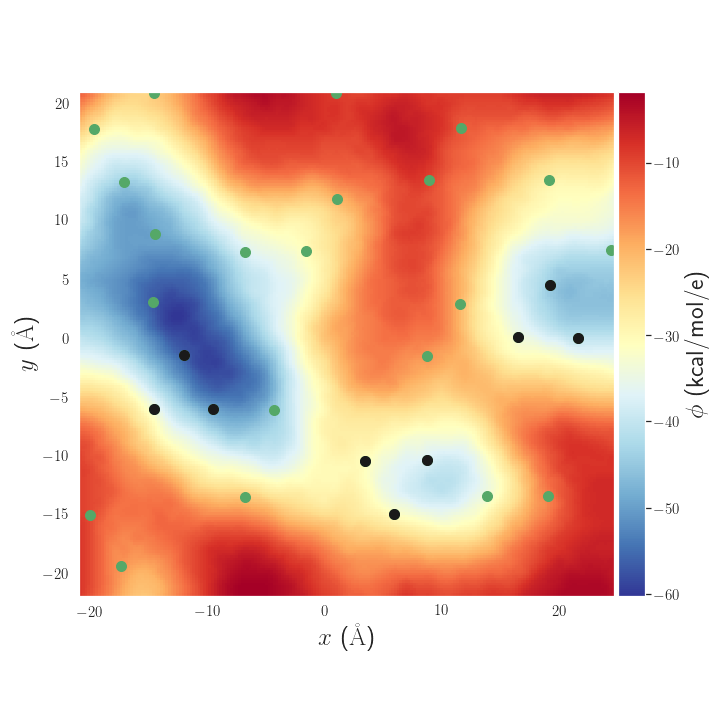
\includegraphics[width=0.75\columnwidth]{./images/erratum_EPS.png}
\caption[Correction to Electrostatic Potential Surface]{Corrected electrostatic potential 
($\phi$) surface at $z=$\SI{-10}{\angstrom} in \si{\kilo\cal\per\mol\per\e} as it should have 
appeared in the article. The published figure had the sign of both axis changed. Mg are 
represented as green circles or black circles if they are part of a site.}
\label{erratum_EPS}
\end{figure}
When preparing the material for the thesis manuscript, I realized that the electrostatic 
potential energy surface published in the article 
of this chapter (Figure 7) was wrong. The correct figure would have had changed signs 
of both the $x$ and $y$ axis. Figure \ref{erratum_EPS} contains the correct information. 

We find that the electrostatic potential is minimum in the regions close to the sites. On the 
contrary to our speculation in the article, the strong interaction with the sites is 
electrostatic. The strength of the interaction is very high which explains the 
low diffusion of the cations. Additionally, the strength of the interaction varies in each 
site due to the different substitution pattern around them. The electrostatic 
potential is screened by the water molecules and the rest of the cations. The strength of this 
screening is different if there is one HI per interlayer or four. The different screening in 
either system explains the difference in cation diffusivity. 

In the section ``Uranyl Diffusion Modeling'', the translational self-diffusion coefficient 
published was mistranscribed. The 
actual value is $D^\text{MD}=0.004\pm0.002\cdot 10^{-5}\si{\centi\meter\squared\per\second}$. 
Fortunately, the parameter that was analyzed, the constrictivity factor was correct.